\documentclass[draft]{article}

% PACKAGES
\usepackage[utf8]{inputenc}
\usepackage{amsmath,amssymb,mathtools}
\usepackage{ntheorem}
\usepackage[margin=4cm]{geometry}
\usepackage[final]{listings}
\usepackage{xcolor, color}
\usepackage{algorithm} % for algorithm environment
\usepackage[final]{graphicx}
\usepackage{setspace}
\usepackage{float}
\usepackage{multirow, multicol}
\usepackage{enumitem}
\usepackage{ifdraft}
\usepackage{xspace}
\usepackage{enumitem}
\usepackage{tabularx,comment}
\usepackage{soul}
\usepackage{scalefnt} % scale font
\usepackage{mdframed} % frame figures
\usepackage{pifont} % tick and cross
\usepackage{parskip} % no indentation and paragraph spacing
\usepackage[pdfpagelabels=true,backref=page,bookmarks=true]{hyperref} % KEEP AT THE END OF THE IMPORTS

\ifdraft{\usepackage[colorinlistoftodos, textwidth = 30mm]{todonotes}}{\usepackage[disable, colorinlistoftodos, textwidth = 30mm]{todonotes}}

% Colors
\definecolor{cred}{rgb}{1, 0.5, 0.5}
\definecolor{cgreen}{rgb}{0.5, 1, 0.5}
\definecolor{cblue}{rgb}{0.5, 0.5, 1}

% Hyperref setup
\hypersetup{
    final=true,
    colorlinks=true,
    linkcolor=cblue,
    urlcolor=cred,
    citecolor=teal,
}

% Draft mode changes:  
% https://tex.stackexchange.com/questions/49277/what-does-the-draft-mode-change
% ===== SETTINGS =====
\pagestyle{plain}

% Margins
\textwidth 18 cm
\textheight 22 cm
\topmargin -1 cm
\oddsidemargin -1 cm

% Directories
\newcommand{\definedir}[2]{\newcommand{#1}{#2}}
\definedir{\secs}{../secs}
\definedir{\figs}{../images}

% Style
\definecolor{codegreen}{rgb}{0,0.6,0}
\definecolor{codegray}{rgb}{0.5,0.5,0.5}
\definecolor{codepurple}{rgb}{0.58,0,0.82}
\definecolor{backcolour}{rgb}{0.95,0.95,0.92}
\lstdefinestyle{mystyle}{
    backgroundcolor=\color{backcolour},   
    commentstyle=\color{codegreen},
    keywordstyle=\color{magenta},
    numberstyle=\tiny\color{codegray},
    stringstyle=\color{codepurple},
    basicstyle=\ttfamily\normalsize,
    breakatwhitespace=false,         
    breaklines=true,                 
    captionpos=b,                    
    keepspaces=true,                 
    numbers=left,                    
    numbersep=5pt,                  
    showspaces=false,                
    showstringspaces=false,
    showtabs=false,                  
    tabsize=2
}
\lstset{style=mystyle}

% Footnote style
\let\svthefootnote\thefootnote
\newcommand\freefootnote[1]{%
  \let\thefootnote\relax%
  \footnotetext{#1}%
  \let\thefootnote\svthefootnote%
}

\setlength{\skip\footins}{2pc}

%Enumerate (1 -> 1.1 -> 1.1.1)
\renewcommand{\labelenumii}{\theenumii}
\renewcommand{\theenumii}{\theenumi.\arabic{enumii}.}

% ===== MACROS =====

% Comments
\newcommand{\todotag}{\sethlcolor{red}\hl{ to-do }\xspace}
\newcommand{\js}[1]{{\todo[size=\small, color=blue!40]{Javier: #1}}}
\newcommand{\jsi}[1]{{\todo[inline, size=\small, color=blue!40]{Javier: #1}}}
\newcommand{\mb}[1]{{\todo[size=\small, color=red!40]{Marta: #1}}}
\newcommand{\mbi}[1]{{\todo[inline, size=\small, color=red!40]{Marta: #1}}}
\newcommand{\dk}[1]{{\todo[size=\small, color=orange!40]{Dmitry: #1}}}
\newcommand{\dki}[1]{{\todo[inline, size=\small, color=orange!40]{Dmitry: #1}}}
\newcommand{\zp}[1]{{\todo[size=\small, color=red!40]{Zaira: #1}}}
\newcommand{\zpi}[1]{{\todo[inline, size=\small, color=green!40]{Zaira: #1}}}
\newcommand{\xs}[1]{{\todo[size=\small, color=red!40]{Xavier: #1}}}
\newcommand{\xsi}[1]{{\todo[inline, size=\small, color=purple!40]{Xavier: #1}}}

% Hyperlinks
\newcommand{\hlset}[1]{\hypertarget{\detokenize{#1}}{#1}}
\newcommand{\hlget}[1]{\hyperlink{\detokenize{#1}}{#1}}

% Mathbb
\newcommand{\N}{\mathbb{N}}
\newcommand{\Z}{\mathbb{Z}}
\newcommand{\E}{\mathbb{E}}
\newcommand{\F}{\mathbb{F}}
\newcommand{\G}{\mathbb{G}}
\newcommand{\Q}{\mathbb{Q}}
\newcommand{\R}{\mathbb{R}}
\newcommand{\J}{\mathbb{J}}
\newcommand{\B}{\mathbb{B}}

% Mathsf
\newcommand{\klic}{\mathsf{k_{lic}}}
\newcommand{\kreq}{\mathsf{k_{req}}}
\newcommand{\kdh}{\mathsf{k_{DH}}}
\newcommand{\ksym}{\mathsf{k}}
\newcommand{\tkdh}{\mathsf{\tilde{k}_{DH}}}
\newcommand{\tklic}{\mathsf{\tilde{k}_{lic}}}
\newcommand{\tkreq}{\mathsf{\tilde{k}_{req}}}
\newcommand{\sk}{\mathsf{sk}}
\newcommand{\pk}{\mathsf{pk}}
\newcommand{\ck}{\mathsf{ck}}
\renewcommand{\pk}{\mathsf{pk}}
\newcommand{\vk}{\mathsf{vk}}
\newcommand{\npk}{\mathsf{npk}}
\newcommand{\user}{\mathsf{user}}
\newcommand{\NFT}{\mathsf{NFT}}
\newcommand{\LP}{\mathsf{LP}}
\newcommand{\SP}{\mathsf{SP}}
\newcommand{\npkn}[1]{\mathsf{npk}_{#1}}
\newcommand{\nsk}{\mathsf{nsk}}
\newcommand{\lsk}{\mathsf{lsk}}
\newcommand{\lpk}{\mathsf{lpk}}
\newcommand{\rpk}{\mathsf{rpk}}
\newcommand{\spk}{\mathsf{spk}}
\newcommand{\tx}{\mathsf{tx}}
\newcommand{\txold}{\mathsf{tx^{old}}}
\newcommand{\txm}{\mathsf{tx_{metadata}}}
\newcommand{\txp}{\mathsf{tx_{payload}}}
\newcommand{\txh}{\mathsf{tx_{hash}}}
\newcommand{\txproof}{\mathsf{tx_{proof}}}
\newcommand{\Note}{\mathsf{N}}
\newcommand{\lic}{\mathsf{lic}}
\newcommand{\req}{\mathsf{req}}
\newcommand{\Session}{\mathsf{session}}
\newcommand{\SessionCookie}{\mathsf{sc}}
\newcommand{\nfthash}{\mathsf{hash_{NFT}}}
\newcommand{\nftpayload}{\mathsf{payload_{NFT}}}
\newcommand{\sig}{\mathsf{sig}}
\newcommand{\lsig}{\mathsf{sig_{lic}}}
\newcommand{\tsig}{\mathsf{sig_{tx}}}
\newcommand{\attr}{\mathsf{attr}}
\newcommand{\sign}{\mathsf{sign\_single\_key}}
\newcommand{\signd}{\mathsf{sign\_double\_key}}
\newcommand{\verify}{\mathsf{verify\_sig\_single\_key}}
\newcommand{\verifyd}{\mathsf{verify\_sig\_double\_key}}
\newcommand{\mintnft}{\mathsf{mint\_nft}}
\newcommand{\NoteB}{\mathsf{N_{B}}}
\newcommand{\NoteC}{\mathsf{N_{C}}}
\newcommand{\nnew}[1]{\mathsf{N^{new}_{#1}}}
\newcommand{\nold}[1]{\mathsf{N^{old}_{#1}}}
\newcommand{\vnew}[1]{\mathsf{v_{#1}}}
\newcommand{\vold}[1]{\mathsf{w_{#1}}}
\newcommand{\change}{\mathsf{change}}
\newcommand{\type}{\mathsf{type}}
\newcommand{\com}{\mathsf{com}}
\newcommand{\enc}{\mathsf{enc}}
\newcommand{\nonce}{\mathsf{nonce}}
\newcommand{\pos}{\mathsf{pos}}
\newcommand{\nullifier}{\mathsf{nullifier}}
\newcommand{\isseen}{\mathsf{is\_seen}}
\newcommand{\pnullifiers}{\mathsf{previous\_nullifiers}}
\newcommand{\sessionid}{\mathsf{session\_id}}
\newcommand{\hb}{H^\mathsf{BLAKE2b}}
\newcommand{\hp}{H^\mathsf{Poseidon}}

% Mathfrak
\newcommand{\Ftuple}{\mathfrak{F}}
\newcommand{\Bitstrings}{\mathfrak{B}}

% Misc maths
\newcommand{\floor}[1]{\lfloor #1 \rfloor}
\newcommand{\ceil}[1]{\lceil #1 \rceil}

% Misc cryptography
\newcommand{\sample}{\xleftarrow{\$}}
\newcommand{\error}{\perp}
\newcommand{\conc}{\;||\;}
\newcommand{\snull}{\sf{null}}

% Building blocks
\renewcommand{\SS}{\sf{S}}
\newcommand{\EE}{\sf{E}}
\newcommand{\CC}{\sf{C}}
\newcommand{\PP}{\sf{P}}
\newcommand{\MT}{\sf{MT}}
\newcommand{\NN}{\sf{N}}

% Cryptographic algorithms
\newcommand{\Setup}{\sf{Setup}}
\newcommand{\SetupU}{\sf{SetupUniversal}} % find a better one
\newcommand{\SetupD}{\sf{SetupDependent}} % find a better one
\newcommand{\Com}{\sf{Com}}
\newcommand{\Hash}{\sf{Hash}}
\newcommand{\Enc}{\sf{Enc}}
\newcommand{\Dec}{\sf{Dec}}
\newcommand{\SDec}{\sf{SymDec}}
\newcommand{\Sign}{\sf{Sign}}
\newcommand{\Prove}{\sf{Prove}}
\newcommand{\Verify}{\sf{Verify}}
\newcommand{\Nul}{\sf{Nullify}}
\newcommand{\Open}{\sf{Open}}
\newcommand{\UpdateCom}{\sf{UpdateCom}}
\newcommand{\UpdateProof}{\sf{UpdateProof}}

% Misc
\newcommand{\secparam}{\sf{security_parameter}}
\newcommand{\vin}{\sf{in}}
\newcommand{\vout}{\sf{out}}
\newcommand{\msg}[1][]{\sf{message}^{#1}}
\newcommand{\accept}{\sf{accept}}
\newcommand{\reject}{\sf{reject}}
\newcommand{\pp}{\sf{pp}}
\newcommand{\crs}{\sf{crs}} % do we need both CRS and SRS?
\newcommand{\srs}{\sf{srs}}
\newcommand{\transfer}{\sf{transfer}}
\newcommand{\length}{\sf{length}}

% State
\newcommand{\holders}{\sf{holders}}
\newcommand{\securities}{\sf{securities}}
\newcommand{\nullifiers}{\sf{usedNullifiers}}
\newcommand{\vmax}{\sf{max}}
\newcommand{\vsupply}{\sf{supply}}
\newcommand{\vlimit}{\sf{limit}}

% Roles
\newcommand{\holder}{\sf{holder}}
\newcommand{\issuer}{\sf{issuer}}
\newcommand{\auditor}{\sf{auditor}}
\newcommand{\sender}{\sf{sender}}
\newcommand{\recipient}{\sf{recipient}}
\newcommand{\viewer}{\sf{viewer}}

% Merkle trees / Merkle proofs
\newcommand{\tree}[1][]{\sf{tree}^{\sf{#1}}}
\renewcommand{\root}[1][]{\sf{root}^{\sf{#1}}}
\newcommand{\recentroots}{\sf{recentRoots}}
\newcommand{\leaf}{\sf{leaf}}
\newcommand{\leaves}{\sf{leaves}}

% Circuits
\newcommand{\inputs}{\sf{input}}
\newcommand{\public}{\sf{public}}
\newcommand{\secret}{\sf{secret}}

% Values
\newcommand{\val}[1][]{\sf{value}^{#1}}

% Keys and key components
\newcommand{\SK}{\sf{SecretKey}}
\newcommand{\PK}{\sf{PublicKey}}
\newcommand{\seed}{\sf{seed}}
\renewcommand{\k}[1][]{\sf{k}^{#1}}
\newcommand{\spend}{\sf{spend}}
\newcommand{\view}{\sf{view}}
\newcommand{\nullify}{\sf{nullify}}
\newcommand{\token}{\sf{token}}

% Securities
\newcommand{\content}[1]{\sf{content}^{#1}}
\newcommand{\blinder}[1][]{\sf{blinder}^{#1}}
\newcommand{\bitmask}[1][]{\sf{bitmask}^{#1}}
\newcommand{\opening}[1][]{\sf{opening}^{#1}}

% Contract methods
\newcommand{\cAdd}{\sf{AddToAllowlist}}
\newcommand{\cRemove}{\sf{RemoveFromAllowlist}}
\newcommand{\cMint}{\sf{Mint}}
\newcommand{\cBurn}{\sf{Burn}}
\newcommand{\cTransfer}{\sf{Transfer}}
\newcommand{\cForced}{\sf{ForcedTransfer}}

% Wallet functionalities
\newcommand{\wKeys}{\sf{CreateKeys}}
\newcommand{\wOutput}{\sf{ComputeOutput}}
\newcommand{\wNul}{\sf{ComputeNullifier}}
\newcommand{\wComTransfer}{\sf{ComputeTransferCommitment}}
\newcommand{\wComSwap}{\sf{ComputeSwapCommitment}}
\newcommand{\wSign}{\sf{ComputeSpendingAuthorization}}
\newcommand{\wMProof}{\sf{ComputeMembershipProof}}
\newcommand{\wProof}{\sf{ComputeTransferProof}}
\newcommand{\wDecViewer}{\sf{DecryptByViewer}}
\newcommand{\wDecOutAuditor}{\sf{DecryptOutputByAuditor}}
\newcommand{\wDecNulAuditor}{\sf{DecryptNullifierByAuditor}}

% Atomic swaps
\newcommand{\maker}{\sf{maker}}
\newcommand{\taker}{\sf{taker}}
\newcommand{\seca}{\sf{A}}
\newcommand{\secb}{\sf{B}}
\newcommand{\secx}{x}
\newcommand{\swap}{\sf{swap}}
\newcommand{\xmax}[1][]{\sf{X}^{#1}}
\newcommand{\contract}[1][]{\sf{contract}^{#1}}
\newcommand{\this}{\sf{this}}
\newcommand{\swapdata}[1][]{\sf{swapData}^{#1}}
\newcommand{\transferdata}[1][]{\sf{transferData}^{#1}}

% Indices
\newcommand{\ai}{\seca, i}
\newcommand{\bi}{\secb, i}
\renewcommand{\xi}{\secx, i}
\newcommand{\fii}{i = 1, 2}
\newcommand{\fio}{i = 3, 4}
\newcommand{\fs}{\secx = \seca, \secb}
\newcommand{\falli}{{\substack{x = \seca, \secb \\ i = 1, 2}}}
\newcommand{\fallo}{{\substack{x = \seca, \secb \\ i = 3, 4}}}

% Entity tags
\newcommand{\tagauditor}{\sethlcolor{yellow}\hl{ auditor }\xspace}
\newcommand{\tagissuer}{\sethlcolor{orange}\hl{ issuer }\xspace}
\newcommand{\tagholders}{\sethlcolor{cyan}\hl{ holders }\xspace}
\newcommand{\tagwhitelisted}{\sethlcolor{brown}\hl{ whitelisted }\xspace}
\newcommand{\tagviewer}{\sethlcolor{lime}\hl{ viewer }\xspace}

% Symbols
\newcommand{\cmark}{\ding{51}}%
\newcommand{\xmark}{\ding{55}}%

% Formatting
\newcommand{\method}[1]{\noindent{#1}}
\newcommand{\textmc}[1]{\textsc{\scalefont{1}#1}}
\newcommand{\tinputs}{\textmc{inputs}{ }}
\newcommand{\tproc}{\textmc{procedure}{ }}
\newcommand{\toutputs}{\textmc{outputs}{ }}
\lstnewenvironment{code}[1][]%
  {\noindent\minipage{\linewidth}\medskip 
   \lstset{basicstyle=\fontsize{8}{8}\selectfont\ttfamily,frame=single,#1,backgroundcolor=\color{white}}}
  {\endminipage}

% Miscallaneous
\newcommand\mut[1]{\ignorespaces}
\renewcommand{\sf}[1]{\ensuremath{\mathsf{#1}}}
\renewcommand{\tt}[1]{\texttt{#1}}

\title{Citadel protocol specification}
\author{Dusk Network}
\date{\today}

\begin{document}
	
\maketitle
\vspace{0.6cm}

\tableofcontents

\newpage

\section{Protocol overview}
\label{sec:general-overview}
% !TeX root = ../build/main.tex

Citadel is a self-sovereign identity (SSI) protocol built on tope of Dusk that allows users of a given service to manage their digital identities in a fully transparent manner. More specifically, every user can know which information about them is shared with other parties, and accept or deny any request for personal information.

\subsection{Properties}

With Citadel, users of a service can request licenses that represent their \emph{right} to use such a service. Citadel satisfies the following properties:

\begin{itemize}
	\item \emph{Proof of ownership}: users can prove that they own a valid license that allows them to use a certain service.
	\item \emph{Proof of validity}: users with a valid license can prove that their license has not been revoked and is valid.
	\item \emph{Unlinkability}: different services used by a same user cannot be linked from one another.
	\item \emph{Decentralized session opening}: when users start using a service, the network learns that this happened and the license used to access to the service cannot be used again.
	\item \emph{Attribute blinding}: users have the power to decide exactly what information they want to share and with whom.
\end{itemize}

\subsection{The parties involved}

Citadel involves three (potentially different) parties:

\begin{itemize}
    \item The \emph{user} is the person who interacts with the wallet and requests licenses in order to claim their right to make use of services.
    \item The \emph{service provider} (SP) is the entity that offers a service to users. Upon verification that a service request from a user is correct, it provides such service.
    \item The \emph{license provider} (LP) is the entity that receives requests for licenses from users, and upon acceptance, issues them. The LP can be the same SP entity or a different one.
\end{itemize}

\subsection{The elements involved}

Below there is the list of the elements involved in the protocol. The details of their structure and their role are explained in the following sections. 

\begin{itemize}
	\item A \emph{request} is a set of information that the user sends to the network in order to inform the LP that they are requesting a license. It includes an stealth address where the license will be sent to.
	\item A \emph{license} is an asset that represents the right of a user to use a certain service. In particular, a license contains a set of attributes that are associated to the requirements needed to make use of that service.
	\item The \emph{LicenseProverParameters} are the set of parameters needed by the user to compute a proof that proves their license ownership.
	\item A \emph{session} is a set of public values sent by the user to the network that are associated with the initiation of the use of a service.
	\item A \emph{session cookie} is a set of values that allows the SP to verify that a session was opened correctly.
\end{itemize}

\subsection{Protocol flow}

{\color{red}[Missing explanation]}

\begin{figure}[h]
	\centering
	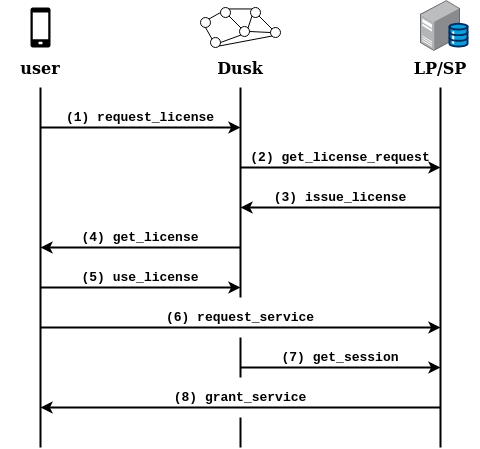
\includegraphics[width=.4\textwidth]{\figs/protocol.png}
	\caption{Overview of the protocol messages exchanged between the user, Dusk's network, and the LP/SP.}
	\label{fig:protocol}
\end{figure}



\section{Cryptographic primitives}
\label{sec:crypto-primitives}
% !TeX root = ../build/main.tex

In this section, we detail the cryptographic primitives used in Citadel. We briefly introduce Merkle trees, the commitment scheme, encryption scheme, proof system, elliptic curves and hash functions used, specifying at each step the concrete parameters with which each of the primitives is instantiated.

\paragraph{Notation.} Throughout the document, we use the following conventions. Given a set $S$, we denote sampling an element $x$ uniformly at random from $S$ by $x\gets S$. Any group $\G$ used is of a large prime order, and we assume that the discrete logarithm problem is hard in $\G$. If two elements are denoted by the same letter in upper case and lower case, e.g. $a, A$, this often signifies the fact that $A$ is a public key corresponding to the secret key $a$. 
%By $\{0,1\}^*$, we denote all bitstrings of arbitrary length.\mb{Add $\F_p$ and $\F_p^*$ notation.}

\subsection{Elliptic curves}\label{sec:elliptic_curves}

BLS12-381~\cite{zcashBLS} and Jubjub~\cite{zcashJubJub} are the elliptic curves used. More precisely, let
\[\begin{array}{lll}
	& q = & 4002409555221667393417789825735904156556882819939007885332058136 \\
	& & 124031650490837864442687629129015664037894272559787,\\
	\\
	& p = & 5243587517512619047944774050818596583769055250052763782260365869 \\
	& & 9938581184513.
\end{array}\]
Note that both are prime numbers, with bit-lengths $381$ and $255$, respectively. The curve BLS381-12 is the curve over $\mathbb{F}_q$ defined by the equation
\[E: Y^2 = X^3 + 4.\]
We have that $E(\mathbb{F}_q)$ has different subgroups $\G_1, \G_2$ such that $\#\G_1 = \#\G_2 = p$. This curve is pairing-friendly (with embedding degree $k=12$), so pairings are efficiently computable. More precisely, Citadel makes use of the bilinear group 
\[\mathbb{B}=\left( p, \G_1, \G_2, \G_T, e: \G_1\times\G_2 \rightarrow \G_T \right).\]

By instantiating the zk-SNARK with the bilinear group $\mathbb{B}$, we are be able to prove statements about satisfiability of arithmetic circuits over $\mathbb{F}_p$, the so-called \emph{scalar field} of $E$. 

Furthermore, we are interested in proving certain operations with the zk-SNARK, like the correct verification of a Schnorr signature $\sigma$. Note that $\sigma$ is an element of a certain elliptic curve $J$, but is represented as two coordinates in the base field $\F_s$ of $J$. Therefore, the verification can be best represented as arithmetic constraints modulo $s$. While it is possible to represent any NP statement using arithmetic modulo $p$ to plug it into the zk-SNARK, this incurs into a significant efficiency loss if not done carefully. The natural thing is to set $s=p$. Therefore, the signature scheme must be instantiated with an elliptic curve over $\mathbb{F}_p$. For this, let
\[d = -\frac{10240}{10241} \bmod{p}.\]
Citadel uses the Jubjub curve, defined by the equation
\[J : -X^2+Y^2 = 1 + dX^2Y^2,\]
over $\mathbb{F}_p$. In particular, it uses a subgroup $\mathbb{J}$ of order
\[\begin{array}{lll}
	& t = & 6554484396890773809930967563523245729705921265872317281365359162 \\
	& & 392183254199,\\
\end{array}\]
which is a $252$-bit prime. 

The primes and groups defined here will be used through the rest of the document.

\subsection{Digital signatures}\label{sec:signatures}

The Schnorr Sigma protocol~\cite{schnorr1989efficient} is used, compiled with the Fiat--Shamir transformation~\cite{fiat1986prove,pointcheval1996security}, as a signature scheme. 
In particular, Citadel makes use of the standard scheme as well as a double-key version to be able to delegate computations later in the protocol. Let $G, G'\gets \mathbb{J}$.

The single-key signature scheme is as follows.

\begin{itemize}
	\item \emph{Setup.} Sample a secret key $\sk \gets \F_t$ and set the corresponding public key $\pk = \sk G$. Output $(\sk, \pk)$. 
	\item \emph{Sign.} On input a message $m$ and a secret key $\sk$, sample $r \gets \F_t$ and compute $R = rG$. Compute the challenge $c = H(m, R)$, and set 
	\[u = r - c \sk.\]
	Output the signature $\sigma = (R, u)$. 
	\item \emph{Verify.} On input a public key $\pk$, message $m$ and signature $\sigma = (R, u)$, compute $c = H(m, R)$ and check whether the following equality holds:
	\[\begin{aligned}
		& R = uG + c \pk, \\
	\end{aligned}\]
	If so, accept the signature, otherwise reject.
\end{itemize}

The double-key signature scheme is as follows.

% \mbi{Consider changing $\nsk, \npk$ to $a, A$.}\jsi{Thought about it, but the problem I see is that $a,A$ have a specific meaning in the protocol, which is different from what would be their meaning here. Maybe $h,H$ or $k,K$? But I'm not sure I like these.}
\begin{itemize}
	\item \emph{Setup.} Sample a secret key $\sk \gets \F_t$ and set the corresponding public key $(\pk, \pk') = (\sk G, \sk G')$. Output $(\sk, (\pk, \pk'))$. 
	\item \emph{Sign.} On input a message $m$ and a secret key $\sk$, sample $r \gets \F_t$ and compute $(R, R') = (rG, rG')$. Compute the challenge $c = H(m, R, R')$, and set 
	\[u = r - c \sk.\]
	Output the signature $\sigma = (R, R', u)$. 
	\item \emph{Verify.} On input a public key $\pk$, message $m$ and signature $\sigma = (R, R', u)$, compute $c = H(m, R, R')$ and check whether the following equalities hold:
	\[\begin{aligned}
		& R = uG + c \pk, \\
		& R' = uG' + c \pk'. \\
	\end{aligned}\]
	If so, accept the signature, otherwise reject.
\end{itemize}

\jsi{The computation of the challenge requires $\F_t$ operations, while we are working on an $\F_p$-circuit. If we are doing tricks to circumvent this, it should be reflected and analyzed in the present document. Also, check what is the code doing.\\}

The signature scheme is existentially unforgeable under chosen-message attacks under the discrete logarithm assumption, in the random oracle model~\cite[Section 12.5.1]{katz2020introduction}. While the Schnorr signature scheme is widely known, the double-key version has not been used before, to the best of our knowledge. In Citadel, as it happens in the Phoenix transaction model \cite{phoenix-doc}, this is leveraged to allow for delegation of proof computations without the need to share one's secret key with the helper.

\subsection{Hash functions}\label{sec:hash_functions}

Citadel uses hash functions $H$ mostly in the case where given $y$, we want to prove knowledge of $x$ such that $H(x)=y$. We will do so with PlonK, which requires statements to be written as arithmetic constraints modulo a large prime number $p$. Most hash function evaluations do not naturally translate to this language, incurring in a big efficiency loss. 
%
To avoid this, the Poseidon hash function~\cite{grassi2021poseidon} $H:\mathfrak{F}_p\rightarrow \F_p$, where $\mathfrak{F}_p$ is the set of tuples of $\F_p$-elements of any length, will be used whenever we compute a hash of which we need to produce a proof. This is because Poseidon is purposefully designed to work with modular arithmetic. 

\subsection{Encryption schemes}\label{sec:encryption}

A symmetric encryption scheme~\cite{duskDmitry} based on Poseidon is also used, as described below.

Poseidon is built by applying the sponge construction~\cite{bertoni2011cryptographic} to a permutation $\pi : \F_p^t \rightarrow \F_p^t$, for $t=r+c$, where
\begin{itemize}
	\item $r$ is the \emph{rate}, i.e. the amount of $\F_p$-elements of the input that can be processed in a call to $\pi$.
	\item $c$ is the \emph{capacity}, which is a part of the permutation that is never output by the hash, and is required for security.
\end{itemize}
The permutation $\pi$ is composed of linear (matrix multiplication over $\mathbb{F}_p$) and non-linear (S-boxes) operations. Some rounds are \emph{full rounds}, and apply S-boxes to the whole input, and others are \emph{partial rounds}, in which an S-box is applied to a single $\F_p$-element.

In this case, Citadel uses \textsc{Poseidon}-128 to target 128-bit security. Following the recommendations of~\cite{grassi2021poseidon}, parameters are set as $r=4$ and $c=1$, so that a hash in the Merkle tree can be computed with a single call to the permutation. Internally, a permutation performs $R_F=8$ full rounds and $R_P=59$ partial rounds, and uses $S(x)=x^5$ as the S-box.

When no proofs involving hashes are required, the BLAKE2 family of hash functions~\cite{rfc7693} is used, which yields better efficiency. In particular, the BLAKE2b hash function is used, since it is optimized for 64-bit platforms.

The encryption scheme~\cite{duskDmitry} is a variation of the one-time pad encryption in the field. It uses Poseidon as a pseudorandom function to extend an agreed-upon symmetric key and encrypt the message. Therefore, the encryption scheme is perfectly secure under the random oracle model. 

Concretely, the encryption works as follows. Given a message in $\mathbb{F}_q^{\ell}$, each $\mathbb{F}_q$-component is added to  the corresponding component of the key. The key is obtained using Poseidon by extending the symmetric-encryption key, which is an elliptic curve point, 
to obtain a key with the same size of the message. The initialization vector contains the two coordinates of the key and a nonce, it is passed to the Poseidon iteration which extends the key and outputs the ciphertext. The sender sends the encryption along with the nonce and the information needed to compute the key, so the receiver can use Poseidon with the same key and nonce to decrypt the message.

\subsection{Commitments}\label{sec:commitments}

As commitment scheme, Citadel uses the Pedersen commitment~\cite{pedersen1991non}, which we now describe. 

\begin{itemize}
	\item \emph{Setup.} Sample and output the commitment key $\ck= (G,G')\gets\mathbb{J}^2$.
	\item \emph{Commit.} On input a value $v$, sample randomness $r\gets\F_t$ and output
	\[c = \mathsf{Com}_\ck(v;r)=vG+rG'.\]
	\item \emph{Open.} Reveal $v,r$. With these, anyone can recompute the commitment and check if it matches $c$.
\end{itemize}

This scheme is perfectly hiding, and computationally binding under the discrete logarithm assumption.

\subsection{Proof systems}\label{sec:proof_system}

Citadel uses the zk-SNARK PlonK~\cite{gabizon2019plonk} as its proof system. PlonK allows anyone to prove satisfiability of any arithmetic circuit modulo a prime. Since arithmetic circuit satisfiability is an NP-complete problem, this proof system will allow us to prove any statement in NP. 
%
PlonK makes use of the KZG polynomial commitment scheme~\cite{kate2010constant}, as described in~\cite{gabizon2019plonk}. This requires instantiating PlonK over a pairing-friendly group, which is described in Section~\ref{sec:elliptic_curves}.

Below is a summary the efficiency of PlonK, for a circuit with $n$ multiplication gates and $\ell$ public inputs.
\begin{itemize}
	\item \emph{Proving time:} $O(n)$ group and field operations. 
	\item \emph{Verification time:} $O(1+\ell)$ group and field operations.
	\item \emph{Proof size:} $O(1)$ group and field elements.
\end{itemize}

PlonK is sound in the algebraic group model~\cite{fuchsbauer2018algebraic}, and statistically zero-knowledge. A complete and explicit description of the scheme can be found in~\cite[Section~8]{gabizon2019plonk}.

\subsection{Merkle trees}\label{sec:merkle_trees}

A \emph{Merkle tree}~\cite{merkle1987digital} is a tree that contains at every vertex the hash of its children vertices. More precisely, we consider a perfect $k$-ary tree of height $h$. The single vertex at level $0$ is called the \emph{root} of the tree, and the $k^{h}$ vertices at level $h$ are called the \emph{leaves}. Given a vertex in level $i$, the $k$ vertices in level $i+1$ that are adjacent to it are called its \emph{children}. Two vertices are each other's \emph{sibling} if they are children of the same vertex.

%\pagebreak

To each vertex in the tree, we will recursively associate a value, starting from the leaves.\footnote{We will often abuse notation and write the vertex to refer to the value associated with the vertex.} Let $H$ be a hash function. 
\begin{itemize}
	\item Level $h$: leaves are initialized to a null value. Through the lifetime of the tree, they will progressively be filled from left to right with values.
	\item Level $0\leq i <h$: each vertex has $k$ children $c_1,\dots, c_k$ at level $i+1$. We set the value of the vertex to $H({c_1}, \dots, {c_k})$. 
\end{itemize}

The tree is updated every time a new value is written into a leaf, by updating the $h+1$ elements in the path from the new value to the root. In particular, this means that the root changes after every update. A nice feature of Merkle trees is that, given a root $r$, it is easy to prove that a value $x$ is in a leaf of a tree with root $r$. The proof works as follows: 
\begin{itemize}
	\item \emph{Prove.} For $i=h,\dots,1$, let $x_i$ be the vertex that is in level $i$ and is in the unique path from $x$ to the root. Let $y_{i, 1},\dots, y_{i, k-1}$ be the $k-1$ siblings of $x_i$. Output
	\[(x, (y_{1,1}, \dots, y_{1,k-1}), \dots, (y_{h,1},\dots,y_{h,k-1})).\]
	\item \emph{Verify}. Parse input as $(x_h, (y_{1,1}, \dots, y_{1,k-1}), \dots, (y_{h,1},\dots,y_{h,k-1}))$, where $x_h$ is the purported value and $y_{i,1},\dots,y_{i,k-1}$ are the purported siblings at level $i$. For $i=h-1,\dots, 0$, compute\footnote{To be precise, the prover also has to send $\lceil\log_2k\rceil$ bits for each level, specifying the position of $x_i$ with respect to its siblings, so that the verifier knows in which order to arrange the inputs of the hash.}
	\[x_i = H\left( x_{i+1}, y_{i+1,1},\dots,y_{i+1,k-1} \right).\] 
\end{itemize}

This allows for proving membership in a set of size $k^h$ by sending $O(kh)$ values. This proof is sound provided that the hash function is collision resistant~\cite[Section 5.6.2]{katz2020introduction}. For our application, we will set $k=4$ and $h=17$.

\section{Protocol}
\label{sec:protocol}
% !TeX root = ../build/main.tex

\mbi{Change BLAKE2 to Poseidon and leave a footnote.}

In this section, we describe the workflow of Citadel in detail.

\begin{enumerate}

\item (\textbf{user}) $\mathsf{request\_license}()$

	\begin{enumerate}
	
		\item Compute a license stealth address $(\lpk, R_{\lic})$ belonging to the user, using the user's own public key, as follows.
			
			\begin{enumerate}
				\item Sample $r$ uniformly at random from $\F_t$.
				\item Compute a symmetric Diffie--Hellman key $\ksym = rA_{\user}$.
				\item Compute a one-time public key $\lpk = \hb(\ksym)G + B_{\user}$.
				\item Compute $R_{\lic} = rG$.
			\end{enumerate}
		
		\item Compute the license secret key $\lsk = \hb(\ksym) + b_{\user}$ and an additional key $\klic = \hp(\lsk)G$. 
		
		\item Compute the request stealth address $(\rpk, R_{\req})$ using the LP's public key, as follows.
			
			\mbi{Consider using different letter instead of $r$...}
			\begin{enumerate}
				\item Sample $r$ uniformly at random from $\F_t$.
				\item Compute a symmetric Diffie--Hellman key $\kreq = rA_{\LP}$.
				\item Compute a one-time public key $\rpk = \hb(\kreq)G + B_{\LP}$.
				\item Compute $R_{\req} = rG$.
			\end{enumerate}
		
		\item Encrypt data using the key $\kreq$: $\enc = \Enc_{\kreq} ((\lpk, R_{\lic})||\klic; \nonce).$
		
			\mbi{Include how the nonce is computed, if it is a random value as well.}
		
		\item Send the following request to the network: $\req = ((\rpk, R_{\req}), \enc, \nonce).$
		
	\end{enumerate}


\item (\textbf{LP}) $\mathsf{get\_license\_request()}$

	The LP checks continuously the network to detect any incoming license requests addressed to them:
	
	\begin{enumerate}
		\item Compute $\tkreq = a_{\LP}R_{\req}$.
		\item Check if $\rpk \stackrel{?}{=} \hb(\tkreq) G + B_{\LP}$.
	\end{enumerate}

\item (\textbf{LP}) $\mathsf{issue\_license()}$
	
	\begin{enumerate}
		\item Upon receiving a request from a user, define a set of attributes $\attr$ representing the license, and compute a digital signature as follows:
				$$\lsig = \sign_{\sk_{\SP}}(\lpk, \attr).$$
		\item Encrypt the signature and the attributes using the license key:
			  	$$\enc = \Enc_{\klic} (\lsig || \attr; \nonce).$$
		\item Send the following license to the network:
				$$\lic = ((\lpk, R_{\lic}), \enc, \nonce, \pos).$$
	\end{enumerate}
	
\item (\textbf{user}) $\mathsf{get\_license()}$

	In order to receive the license, the user must scan all incoming transactions the following way:
	
	\begin{enumerate}
		\item Compute $\tklic = \hb(\lsk)G$.
		\item Check if $\lpk \stackrel{?}{=} \hb(\tklic) G + B_{\user}$, 
	\end{enumerate}	
	
\item (\textbf{user}) $\mathsf{use\_license()}$

	When using the license, open a session with a specific SP by executing a call to the license contract. The following steps are performed:
	
	\mbi{We should mention something about the license contract before this step. Maybe in Section 2 where elements are presented? Add a small section about Dusk's blockchain?}
	%or something like: the actions performed by the user are interactions with a wallet software, etc. (add part of Milosz' explanation there - or leave it to implementation details).
	%discuss this with Xavi.
	
	\begin{itemize}
		\item The user issues a transaction that calls the license contract, which includes a ZKP that is computed out of the gadget depicted in Figure \ref{fig:circuit_prove_nft}. Notice that here, the user signs $\mathsf{session\_hash}$ using $\lsk$. Likewise, the user here will need to compute $\lpk' = \lsk G'$.
		\item The network validators will execute the smart contract, which verifies the proof. Upon success, the following session will be added to a shared list of sessions:
		
		$$\Session = \{\mathsf{session\_hash}, \sessionid, \com_0^{hash}, \com_1, \com_2\},$$
		
		where $\mathsf{session\_hash} = \hp(\pk_{\SP} || r_\mathsf{session})$, and $r_\mathsf{session}$ is sampled uniformly at random from $\F_t$.
		
		
	\end{itemize}
	
\item (\textbf{user}) $\mathsf{request\_service()}$

Request the service to the SP, establishing communication using a secure channel, and providing the session cookie that follows.
	
	$$\SessionCookie = \{\pk_{\mathsf{SP}}, r_\mathsf{session}, \sessionid, \pk_{\LP}, \attr, c, \mathsf{s_0}, \mathsf{s_1}, \mathsf{s_2}\}$$
	
\item (\textbf{SSP}) $\mathsf{get\_session()}$

Receive a $\Session$ from the list of sessions, where $\Session.\sessionid = \SessionCookie.\sessionid$.
	
\item (\textbf{SSP}) $\mathsf{grant\_service()}$

Grant or deny the service upon verification of the following steps:
	
	\begin{itemize}
		\item Check whether the values $(\attr, \pk_{\LP}, c)$ included in the $\SessionCookie$ are correct.
		\item Check whether the opening $(\pk_{\SP}, r_\mathsf{session})$ included in the $\SessionCookie$ matches the $\mathsf{session\_hash}$ found in the $\Session$.
		\item Check whether the openings $((\pk_{\LP}, \mathsf{s_0}), (\attr, \mathsf{s_1}), (c, \mathsf{s_2}))$ included in the $\SessionCookie$ match the\\
			  commitments ($\com_0^{hash}, \com_1, \com_2$) found in the $\Session$.
	\end{itemize}

\end{enumerate}
	
%\begin{figure}[h]
%	\centering
%	\setlength{\fboxsep}{5pt}%
%	\setlength{\fboxrule}{0.3pt}%
%	\fbox{
%		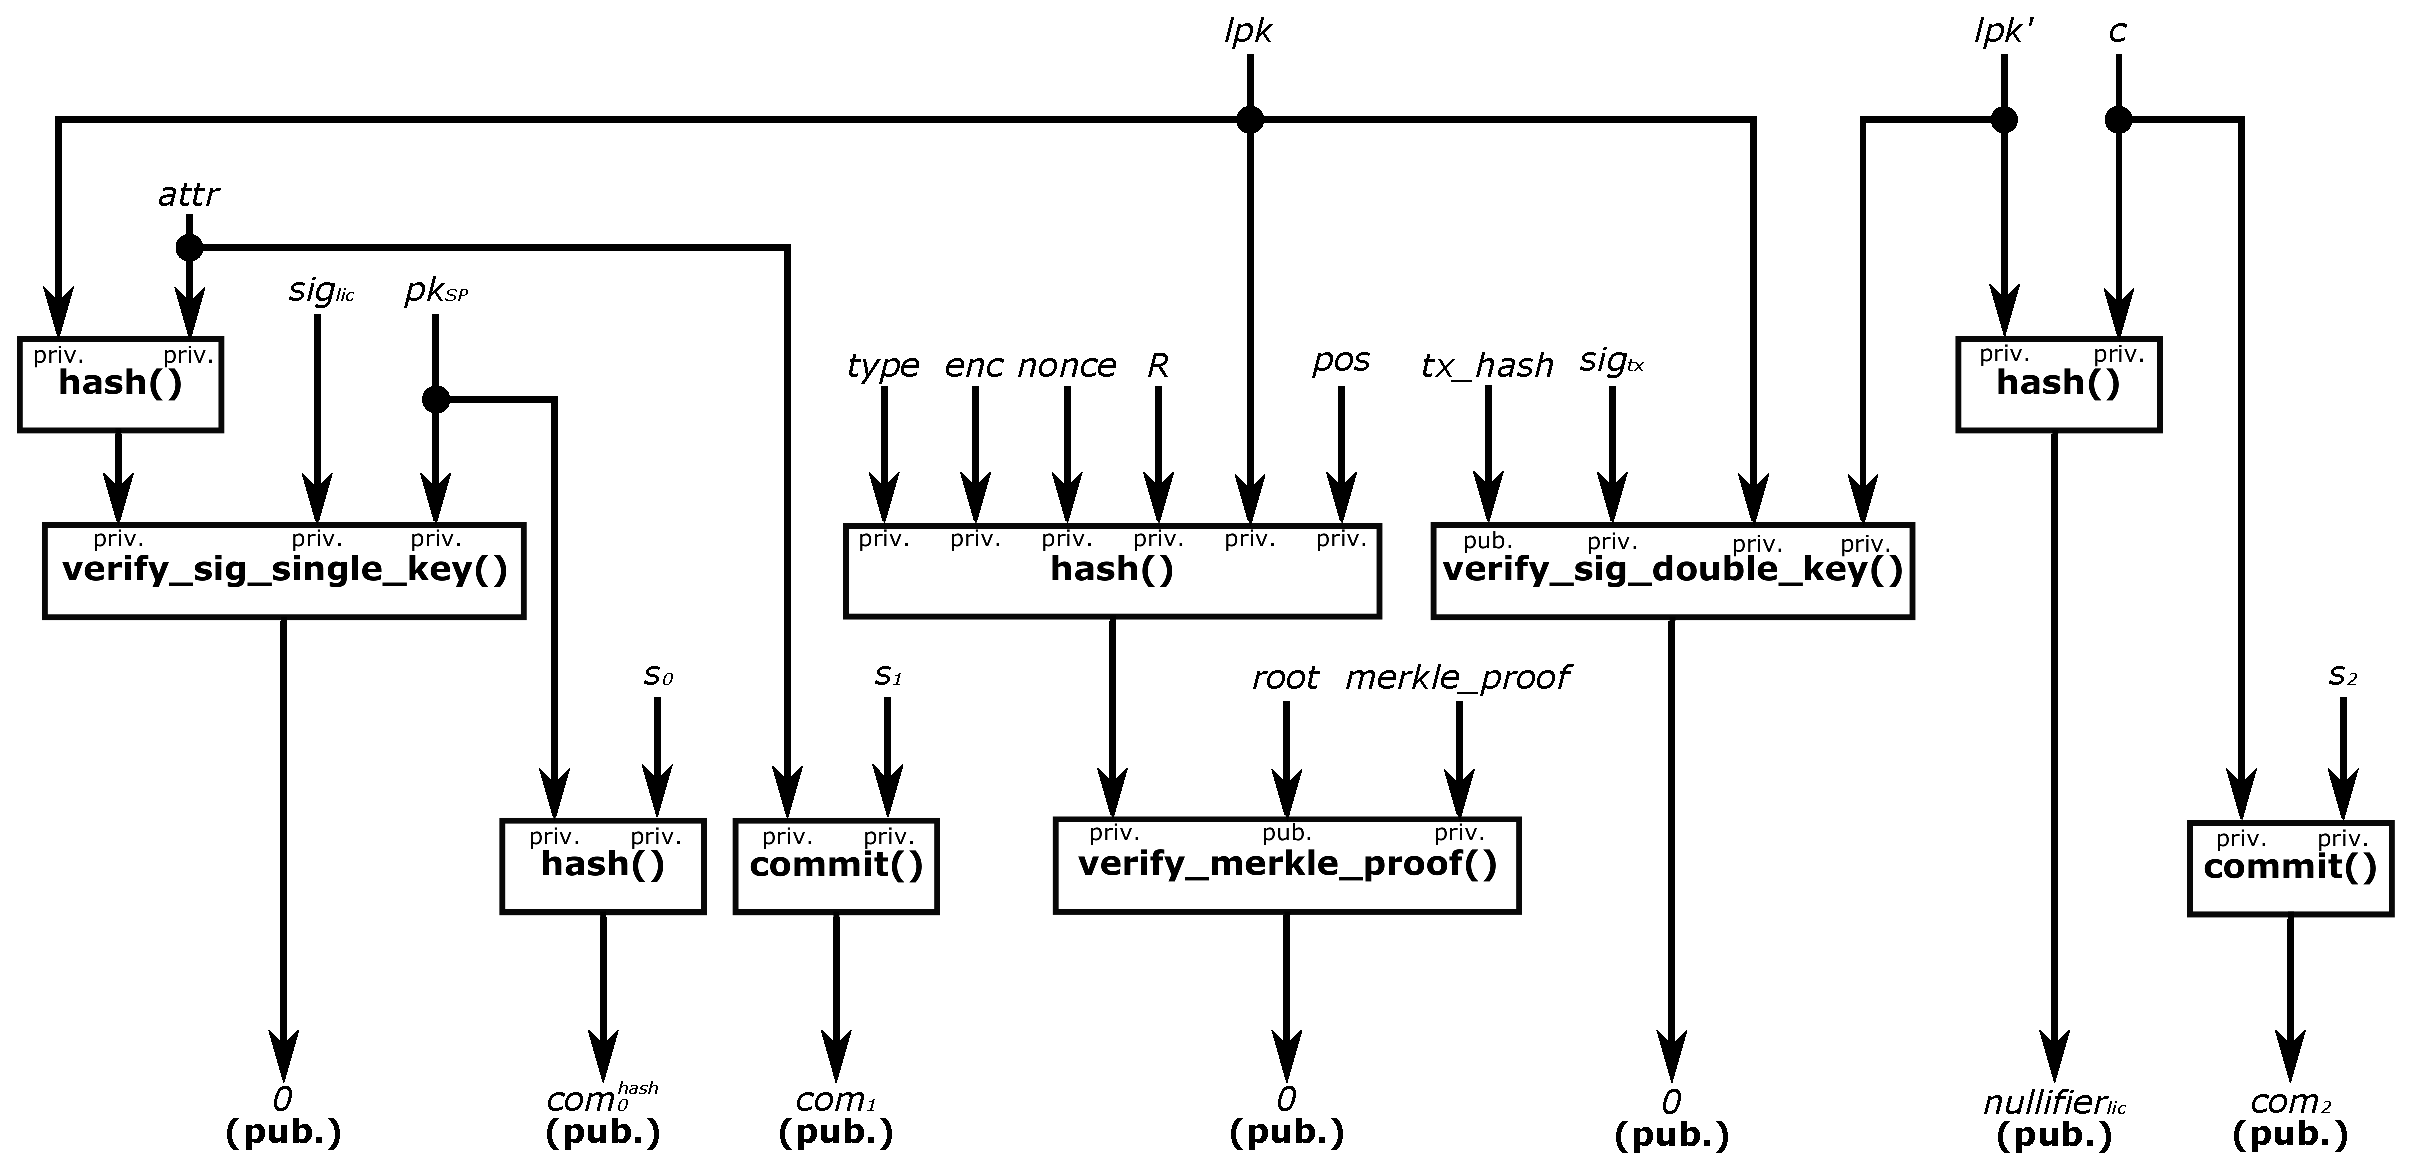
\includegraphics[width=460pt,draft=false]{images/circuit_prove_nft.eps}}
%	\caption{Arithmetic circuit for proving a license's ownership.}
%	\label{fig:circuit_prove_nft}
%\end{figure}

Furthermore, the SP might want to prevent the user from using the license more than once (e.g. this is a single-use license, like entering a concert). This is done through the computation of $\sessionid$. The deployment of this part of the circuit has two different possibilities:
\begin{itemize}
	\item If we set $c = 0$ (or directly remove this input from the circuit), the license can be used only once.
	\item If the SP requests the user to set a custom value for $c$ (e.g. the date of an event), the license can be reused only under certain conditions.
\end{itemize}



\section{Implementation details}
\label{sec:implementation}

\subsection{Participants} 
Protocol implementation involves realization of the protocol building blocks as well as providing means of data communication between them. Building blocks are placed at the following locations, which correspond to protocol participants:

\begin{itemize}%[label=$\bullet$]
	\item User software.
	\item License Provider software.
	\item Service Provider software.
	\item License contract.
\end{itemize}

\begin{flushleft}
Data communication between protocol participants is realized in the following modes:
\end{flushleft}

\begin{itemize}%[label=$\bullet$]
	\item Calling a contract state changing method.
	\item Calling a contract state querying method (not modifying the contract state).
	\item Storing data directly in blockchain.
	\item Retrieving data from blockchain.
	\item Delegating ZK proof calculation.
	\item Calling off-chain.
\end{itemize}

\begin{flushleft}
The following diagram illustrates an interaction between protocol participants and indicates the communication means used.
\end{flushleft}

\begin{figure}[h]
	\centering
		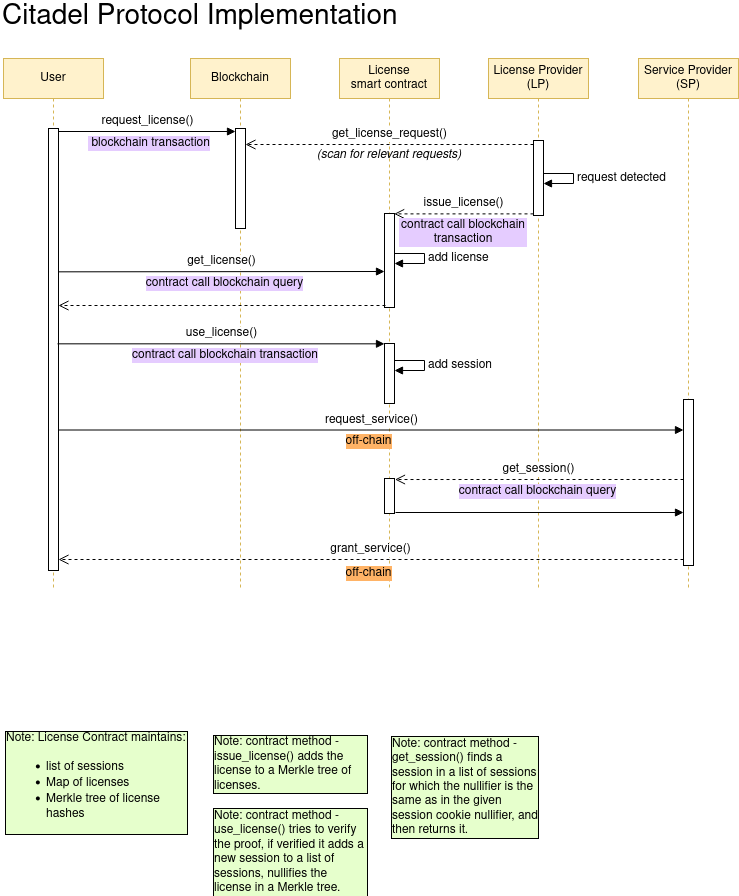
\includegraphics[width=390pt,draft=false]{images/implementation.png}
	\caption{Interaction between protocol participants}
	\label{fig:implementation}
\end{figure}

\begin{flushleft}
On the diagram, we can see various communication modes being used. Initially, the user submits to the blockchain a transaction which contains request as a payload. Subsequently, the License Provider, which continuously scans the blockchain, detects transactions containing requests and filters out requests which are addressed to it. The License Provider can obtain requests via other routes as well, for example via http or email, passing requests on the blockchain is only one of many possible ways of submitting a request, one that has the advantage of passing a payment along with the request. Once the License Provider gets a hold of a request, it can perform appropriate verification, and upon successful verification, it can issue a license. Issuing a license involves a smart contract transaction call. Smart contract transaction call is a blockchain transaction, yet to not confuse the reader, we show it on the diagram with details of blockchain involvement omitted. The user obtains licenses via a contract query. For privacy reasons, the user obtains a bulk of licenses not pertaining exclusively to her and filters it out by herself. To economize the volume of data transfers, block-height range is passed to allow for tranfer of a subset of available records. All modes of communication used so far were on-chain. Communication between the user and the Service Provider, on the other hand, is off-chain. When the Service Provider wants to establish a session, it calls a contract to obtain a session for the given session id.
\end{flushleft}

The diagram illustrates the following flow of data and interactions between participants:

\begin{itemize}%[label=$\bullet$]
	\item User submits request to a License Provider by issuing a blockchain transaction.
	\item License Provider scans the blockchain and obtains the request.
	\item License Provider, upon necessary verification, issues a license.
	\item License Provider sends license to the License Contract via a smart contract call transaction.
	\item User obtains licenses for a given block-height range.
	\item User filters out licenses addressed to her/him.
	\item User calculates a proof (the proof calculation might be delegated).
	\item User calls \textit{use-license} to redeem a license, via a smart contract call.
	\item License Contract attempts to verify the proof and, if verified, adds a new session to a list of sessions.
	\item User requests a service from a Service Provider (off-chain).
	\item Service Provider asks contract for a session.
	\item Service Provider grants service to the user (off-chain).
\end{itemize}


\subsection{License Contract}

\begin{flushleft}
License contract maintains state consisting of the following data:
\end{flushleft}

\begin{itemize}%[label=$\bullet$]
	\item List of sessions.
	\item Map of licenses and their positions in the Merkle tree.
	\item Merkle tree of license hashes.
\end{itemize}


\begin{flushleft}
Contract provides the following methods:
\end{flushleft}

\begin{itemize}%[label=$\bullet$]
	\item \textit{issue-license}: adds a license to a Merkle tree of licenses.
	\item \textit{get-licenses}: provides a list of new licenses added in a given block-height range.
	\item \textit{use-license}: attempts to verify the proof and, if verified, adds a new session to a list of sessions and nullifies the license in the Merkle tree.
	\item \textit{get-session}: finds a session in a list of sessions and returns it to the caller.
\end{itemize}


\subsection{License ZK Proof Calculation}

License ZK proof calculation will either be performed by the user or delegated to a node. At the time of writing, the details of delegation are not yet known, they will be filled in here once the information becomes available.


%\section{Abstract protocol}
%\label{sec:protocol-abstract}
%\input{\secs/protocol-abstract}
%
%\section{Concrete protocol}
%\label{sec:protocol-concrete}
%\input{\secs/protocol-concrete}

\bibliographystyle{splncs04.bst}
\bibliography{biblio.bib}

\end{document}
